% mainfile: ../../main.tex
\chapter{The \pyspeck software package}\label{ch:speck:software}
\lettrine[lines=1]{I}{n} this chapter, I will lay out the design and functionality of the \pyspeck \python package.\sidenote{
    The package repository is hosted on \href{https://git.rwth-aachen.de/qutech/python-spectrometer/}{GitLab}.
    Its documentation is automatically generated and hosted on \href{https://qutech.pages.rwth-aachen.de/python-spectrometer/}{GitLab} as well.
    Releases are automatically published to \href{https://pypi.org/project/python-spectrometer/}{PyPI} and allow the package to be installed using \code{pip install python-spectrometer}.
}

\begin{margintable}
    \footnotesize
    \centering
    \setmintedinline[Python]{fontsize=\footnotesize}
    \caption[Overview of spectrum estimation parameters]{
        Variable names used in \cref{ch:speck:theory} and their corresponding parameter names as used in \pyspeck and \code{scipy.signal.welch()}~\cite{WelchScipy}.
    }
    \label{tab:software:parameters}
    \begin{tabular}{ c C }
        \toprule
        Variable & Parameter \\
        \midrule
        $L$ & n_pts \\
        \fs & fs \\
        $K$ & noverlap \\
        $N$ & nperseg \\
        $M$ & n_seg \\
        \fmin & f_min \\
        \fmax & f_max \\
        \bottomrule
    \end{tabular}
\end{margintable}

\section{Package design and implementation}\label{sec:speck:software:design}
The \pyspeck package provides a central class, \code{Spectrometer}, that users interact with to perform data acquisition, spectrum estimation, and plotting.
It is instantiated with an instance of a child class of the \code{DAQ} base class that implements an interface to various \gls{daq} hardware devices.
New spectra are obtained by calling the \code{Spectrometer.take()} method with all acquisition and metadata settings.

In the following, I will go over the the design of these aspects of the package in more detail.

\subsection{Data acquisition}\label{subsec:speck:software:design:daq}
The \code{daq} module contains on the one hand the declaration of the \code{DAQ} abstract base class and its child class implementations, and on the other the \code{settings} module, which defines the \code{DAQSettings} class.
This class is used in the background to validate data acquisition settings both for consistency (\cf \cref{subsec:speck:theory:welch:parameters}) and hardware constraints.

To better understand the necessity of this functionality, consider the typical scenario of a physicist\sidenote{
    Let's call her Alice.
}
in the lab.
Alice has wired up her experiment, performed a first measurement, and to her dismay discovered that the data is too noisy to see the sought-after effect.
She sets up the \pyspeck code to investigate the noise spectrum of her measurement setup.
From her noisy data she could already estimate the frequency of the most harrowing noise, so she knows the frequency band $[\fmin, \fmax]$ she is most interested in.
But because she is lazy,\sidenote{
    Physicists generally are.
}
she does not want to do the mental gymnastics to convert \fmin to the parameter that her \gls{daq} device understands, $L$ (see \cref{tab:software:parameters}), especially considering that $L$ depends on the number of Welch averages and the overlap.
Furthermore, while she could just about do the conversion from \fmax to the other relevant \gls{daq} parameter, \fs, in her head, her device imposes hardware constraints on the allowed sample rates she can select!
The \code{DAQSettings} class addresses these issues.
It is instantiated with any subset of the parameters listed in \cref{tab:software:parameters}\sidenote{
    \code{DAQSettings} inherits from the builtin \code{dict} and as such can contain arbitrary other keys besides those listed in \cref{tab:software:parameters}.
    However, automatic validation of parameter consistency is only performed for these special keys.
}
and attempts to resolve the parameter interdependencies lined out in \cref{subsec:speck:theory:welch:parameters} upon calling \code{DAQSettings.to_consistent_dict()}.\sidenote{
    Since the graph spanned by the parameters is not acyclic, this only works \emph{most} of the time.
}
This either infers those parameters that were not given from those that were or, if not possible, uses a default value.
Child classes of the \code{DAQ} class can subclass \code{DAQSettings} to implement hardware constraints such as a finite set of allowed sampling rates or a maximum number of samples per data buffer.

For instance, Alice might want to measure the noise spectrum in the frequency band $[\qty{1.5}{\hertz}, \qty{72}{\kilo\hertz}]$.
Although she would not have to do this explicitly,\sidenote{
    Settings are automatically parsed when passed to the \code{take()} method of the \code{Spectrometer} class.
}
she could inspect the parameters after resolution using the code shown in \cref{lst:speck:daq_settings}.

\begin{listing}[htpb]
    \begin{py}
        >>> from python_spectrometer.daq import DAQSettings
        >>> settings = DAQSettings(f_min=1.5, f_max=7.2e4)
        >>> settings.to_consistent_dict()
        {'f_min': 1.5,
         'f_max': 72000.0,
         'fs': 144000.0,
         'df': 1.5,
         'nperseg': 96000,
         'noverlap': 48000,
         'n_seg': 5,
         'n_pts': 288000,
         'n_avg': 1}
    \end{py}
    \caption{
        \code{DAQSettings} example showcasing automatic parameter resolution.
        \code{n_avg} determines the number of outer averages, \ie, the number of data buffers acquired and processed individually.
    }
    \label{lst:speck:daq_settings}
\end{listing}

\begin{marginlisting}
    \begin{py}[fontsize=\footnotesize]
    {'f_min': 14.30511474609375,
     'f_max': 72000.0,
     'fs': 234375.0,
     'df': 14.30511474609375,
     'nperseg': 16384,
     'noverlap': 0,
     'n_seg': 1,
     'n_pts': 16384,
     'n_avg': 1}
    \end{py}
    \caption[Resolved \code{DAQSettings} for MFLI Scope]{
        Resolved settings for the same input parameters as in \cref{lst:speck:daq_settings} but for the \code{ZurichInstrumentsMFLIScope} backend with hardware constraints on \code{n_pts} and \code{fs}. % for some reason tex errors for \code{fs}
    }
    \label{lst:speck:daq_settings:mfli_scope}
\end{marginlisting}
If the instrument she'd chosen for data acquisition had been a Zurich Instruments MFLI's \enquote{Scope} module~\sidecite{ScopeModuleZhinst}, the same requested settings would have resolved to those shown in \cref{lst:speck:daq_settings:mfli_scope}.\sidenote{
    And issued a warning to inform the user their requested settings could not be matched.
}
This is because the Scope module constrains $L\in[2^{12},2^{14}]$ and $\fs\in\qty{60}{\mega\hertz}\times 2^{[-16, 0]} \approx \allowbreak \lbrace \qty{915.5}{\hertz}, \allowbreak \dotsc, \allowbreak \qty{30}{\mega\hertz}, \qty{60}{\mega\hertz}\rbrace$.

As already mentioned, the \code{DAQ} base class implements a common interface for different hardware backends, allowing the \code{Spectrometer} class to be hardware agnostic.
That is, changing the instrument that is used to acquire the data does not necessitate adapting the code used to interact with the instrument.
To enable this, different instruments require small wrapper drivers that map the functionality of their actual driver onto the interface dictated by the \code{DAQ} class.
This is achieved by subclassing \code{DAQ} and implementing the \code{DAQ.setup()} and \code{DAQ.acquire()} methods.
Their functionality is best illustrated by the internal workflow.
When acquiring a new spectrum, all settings supplied by the user are first fed into the \code{setup()} method where instrument configuration takes place.
The method returns the actual device settings,\sidenote{
    Which might differ from the requested settings as outlined above.
}
which are then forwarded to the \code{acquire()} generator function.
Here, the instrument is armed (if necessary), and subsequently data is fetched from the device and yielded to the caller \code{n_avg} times, where \code{n_avg} is the number of outer averages.
\Cref{lst:speck:daq_workflow} represents the data acquisition workflow as pseudocode.

\begin{listing}
    \begin{py}
        daq = SomeDAQ(driver)
        parsed_settings = daq.setup(**user_settings)
        acquisition_generator = daq.acquire(**parsed_settings)
        for data_buffer in acquisition_generator:
            do_something_with(data_buffer)
    \end{py}
    \caption[\gls{daq} workflow pseudocode]{
        \gls{daq} workflow pseudocode.
        A \code{SomeDAQ} object (representing the instrument \code{Some}) is instantiated with a driver object (for instance a \qcodes \code{Instrument}).
        The instrument is configured with the given \code{user_settings}.
        Calling the generator function \code{daq.acquire()} with the actual device settings returns a generator, iterating over which yields one data buffer per iteration.
        The data buffers can then be passed to further processing functions (the \gls{psd} estimator in our example).
    }
    \label{lst:speck:daq_workflow}
\end{listing}
\todo{DAQ pseudocode?}

\subsection{Data processing}\label{subsec:speck:software:design:processing}
\todo{Introduce Bob?}
Once time series data has been acquired using a given \code{DAQ} backend, it could in principle immediately be used to estimate the \gls{psd} following \cref{eq:speck:psd:bartlett}.
However, it is often desirable to transform, or process, the data in some fashion.
This can include simple transformations such as accounting for the gain of a \gls{tia} and convert the voltage back to a current,\sidenote{
    Although it is of course less than trivial to discriminate between current and voltage noise in a \gls{tia}.
}
or more complex ones such as applying calibrations.
In particular, since the process of computing the \gls{psd} already involves Fourier transformation, the processing can also be performed in frequency space.

\begin{marginlisting}
    \begin{py}[fontsize=\footnotesize]
        def compensate_gain(x, gain=1.0):
            return x / gain
    \end{py}
    \caption[Simple \code{procfn} example]{A simple \code{procfn}, which converts amplified data back to the level before amplification.}
    \label{lst:speck:procfn}
\end{marginlisting}
\begin{marginlisting}
    \begin{py}[fontsize=\footnotesize]
        def derivative(xf, f, n=0):
            return xf / (2j * pi * f)**n
    \end{py}
    \caption[Simple \code{fourier_procfn} example]{A simple \code{fourier_procfn}, which calculates the \mbox{(anti-)}derivative.}
    \label{lst:speck:fourier_procfn}
\end{marginlisting}

In \pyspeck, this can be done using a \code{procfn} (in the time domain) or \code{fourier_procfn} (in the Fourier domain).
The former is specified as an argument directly to the \code{Spectrometer} constructor.
It is a callable with signature \code{(x, **kwargs) -> xp}, that is, takes the time series data as its first (positional) argument and arbitrary settings that are passed through from the \code{take()} method as keyword arguments, and returns the processed data.
\Cref{lst:speck:procfn} shows a simple function that accounts for the gain of an amplifier.

The latter is specified in the \code{psd_estimator} argument of the \code{Spectrometer} constructor.
This argument allows the user to specify a custom estimator for the \gls{psd}, in which case a callable is expected.
Otherwise, it should be a mapping containing parameters for the default \gls{psd} estimator, \code{scipy.signal.welch()}~\sidecite{WelchScipy}.
Here, the keyword \code{fourier_procfn} should be a callable with signature \code{(xf, f, **kwargs) -> (xfp, fp)}.\sidenote{
    \Ie, the \code{psd_estimator} argument would be \code{{"fourier_procfn": fn}}.
}
That is, it should take the frequency-space data, the corresponding frequencies, and arbitrary keyword arguments and return a tuple of the processed data and the corresponding frequencies.
The latter are required in case the function modifies the frequencies.\sidenote{
    One example is the \code{octave_band_rms()} function from the \code{qutil.signal_processing} module~\cite{OctaveBandRmsQutil}
}
A simple example for a processing function in Fourier space is shown in \cref{lst:speck:fourier_procfn}, which computes the \mbox{(anti-)}derivative of the data using the fact that
\begin{align}\label{eq:speck:fourier_derivative}
    \pdv[n]{t} \xrightarrow{\mathrm{F.T.}} \left(\i\omega\right)^n
\end{align}
under the Fourier transform.
In \cref{part:setup}\todo{ref}, I discuss more complex use-cases of the processing functionality included in \pyspeck in the context of vibration spectroscopy.

\section{Feature overview}\label{sec:speck:software:features}
\todo{überleitung}
\subsection{Sequential spectrum acquisition}\label{subsec:speck:software:features:sequential}
Now that we have a basic understanding of the design choices underlying \pyspeck, let us discuss the typical workflow of using the package.
The default mode for spectrum acquisition using \pyspeck revolves around the \code{take()} method.
Key to this workflow is the idea that each acquired spectrum can be assigned a comment that allows to easily identify a spectrum in the main plot.
For instance, this comment could contain information about the particular settings that were active when the spectrum was recorded, or where a particular cable was placed.

Consider as an example the procedure of \enquote{noise hunting}, \ie, debugging a noisy experimental setup.
The experimentalist,\sidenote{
    Let's call him Charlie.
}
having discovered that his data is noisier than expected, sets up the \code{Spectrometer} class with an instance of the \code{DAQ} subclass for the \gls{daq} instrument connected to his sample.
Choosing the frequency bounds, say $\fmin = \qty{10}{\hertz}$ and $\fmax = \qty{100}{\kilo\hertz}$, and using the sensible defaults for the remaining spectrum parameters, Charlie first grounds the input of his \gls{daq} to record a \emph{baseline} spectrum.
Thus far, his code would hence look something like that shown in \cref{lst:speck:workflow:sequential}

\begin{listing}
    \begin{py}
        from python_spectrometer import Spectrometer, daq
        from qutil.functools import scaled

        mfli_daq = daq.ZurichInstrumentsMFLIDAQ(session, device)
        spect = Spectrometer(mfli_daq, procfn=scaled(1e6),
                             processed_unit='μV')
        spect.take('baseline', f_min=1e1, f_max=1e5)
    \end{py}
    \caption[\pyspeck workflow]{
        Setup and workflow using the \pyspeck package.
        \code{session} and \code{device} are \gls{api} objects of the \code{zhinst.toolkit} driver package.
        It is therefore possible to simply use the driver objects that are already in use in the measurement setup.
        The \code{procfn} and \code{processed_unit} arguments help converting raw data into a more human-friendly unit.
    }
    \label{lst:speck:workflow:sequential}
\end{listing}

Having obtained a baseline for subsequent experiments, he starts to tweak things on his setup, test out different parameters, \etc
Every time he changes something, he acquires another spectrum using \code{take()}, labeling each with a meaningful comment for identification.

\begin{figure}
    \centering
    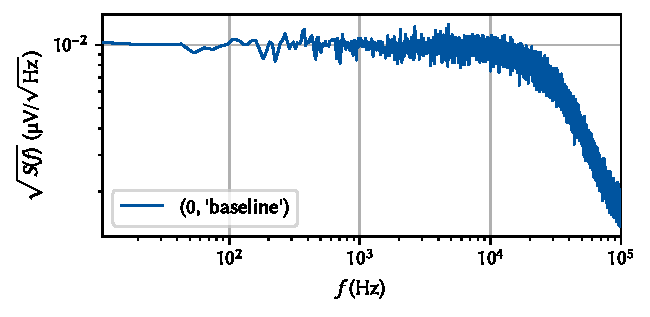
\includegraphics{pdf/spectrometer/workflow_baseline}
    \caption{
        The \pyspeck plot after acquiring the (synthetic) baseline spectrum.
        By default, the \gls{asd} = √\gls{psd} is displayed in the main plot.
    }
    \label{fig:speck:software:workflow_baseline}
\end{figure}

\begin{figure}
    \centering
    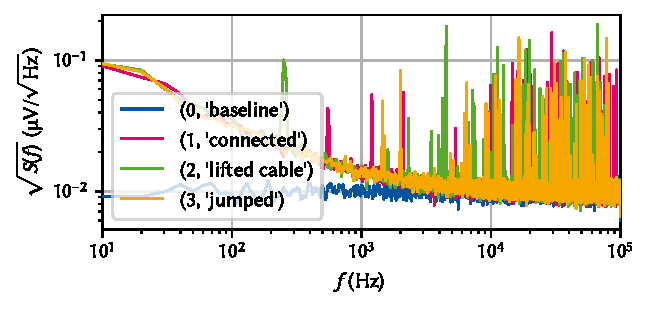
\includegraphics{pdf/spectrometer/workflow_spectra}
    \caption{
        The \pyspeck plot after acquiring additional (synthetic) spectra.
        Each spectrum is uniquely identified by a two-tuple of \code{(index, comment)}.
    }
    \label{fig:speck:software:workflow_spectra}
\end{figure}

\begin{figure}
    \centering
    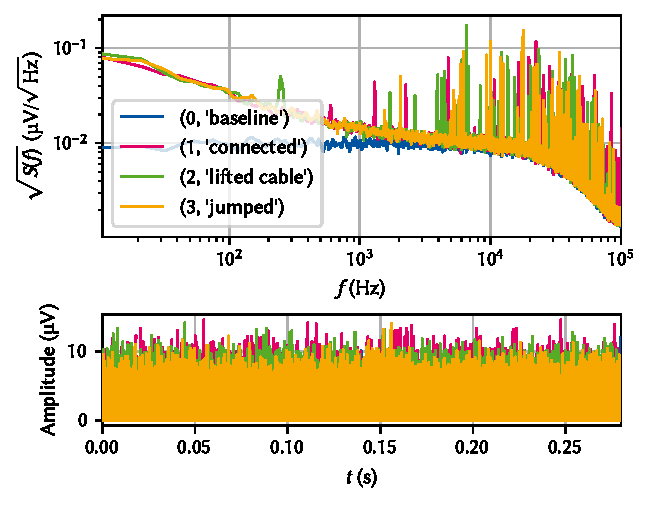
\includegraphics{pdf/spectrometer/workflow_timetrace}
    \caption{
        The \pyspeck plot shown in \cref{fig:speck:software:workflow_spectra} when setting \code{spect.plot_timetrace = True}.
        This adds a subplot that shows the time series data from which the \gls{psd} was computed, \ie, what an oscilloscope would show.
    }
    \label{fig:speck:software:workflow_timetrace}
\end{figure}

\begin{figure}
    \centering
    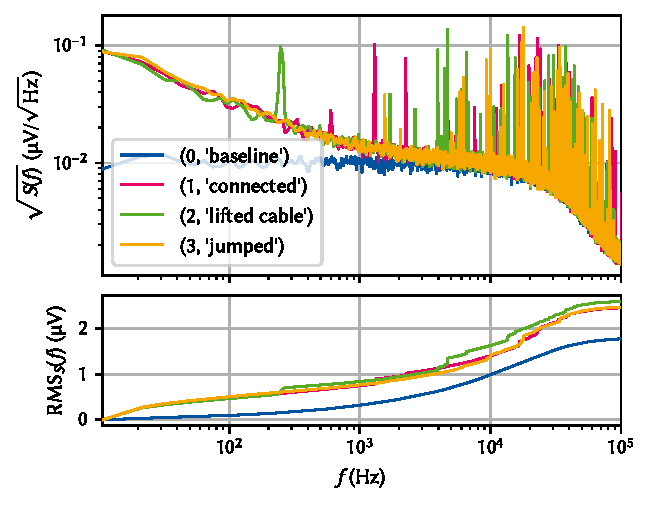
\includegraphics{pdf/spectrometer/workflow_cumulative}
    \caption{
        The \pyspeck plot shown in \cref{fig:speck:software:workflow_spectra} when setting \code{spect.plot_cumulative = True}.
        This adds a subplot that shows the \gls{rms} (\cf \cref{eq:speck:psd:bandpower}) which can be helpful in evaluating the contribution of individual peaks in the spectrum to the total noise power.
        Both the oscilloscope subplot (\cref{fig:speck:software:workflow_timetrace}) and the \gls{rms} subplot can be shown at the same time.
    }
    \label{fig:speck:software:workflow_cumulative}
\end{figure}

\begin{figure}
    \centering
    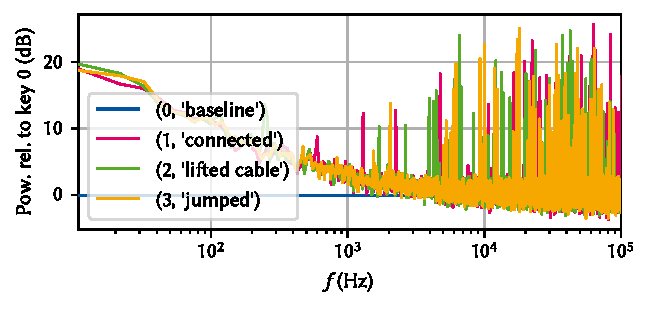
\includegraphics{pdf/spectrometer/workflow_db}
    \caption[The \pyspeck plot in relative mode.]{
        The \pyspeck plot in relative mode.
        Starting from the state in \cref{fig:speck:software:workflow_spectra}, we set \code{spect.plot_dB_scale = True} and \code{spect.plot_amplitude = False} to compare the relative noise powers with respect to the baseline.
    }
    \label{fig:speck:software:workflow_db}
\end{figure}

\begin{figure}
    \centering
    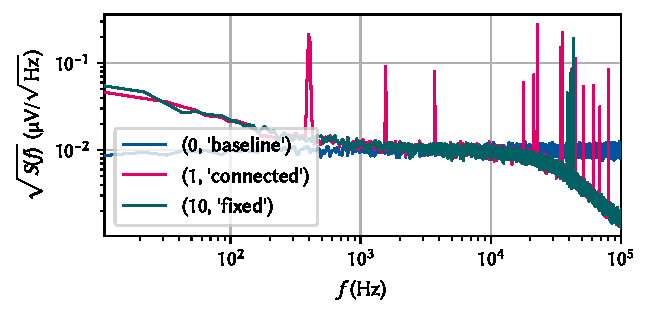
\includegraphics{pdf/spectrometer/workflow_success}
    \caption{
        The \pyspeck plot after multiple additional spectra were acquired and hidden.
        Hiding spectra that one is not interested in anymore is achieved through \code{spect.hide(*range(2, 10))}.
        This is reversed by \code{spect.show(*range(2, 10))}.
        Data can also be dropped (\code{spect.drop(key)}) or deleted (\code{spect.delete(key)}) from the internal cache and disk, respectively.
    }
    \label{fig:speck:software:workflow_success}
\end{figure}



Having acquired six more spectra in between, he hides those he is not interested in anymore from the plot using \code{spect.hide(*range(2, 10))}.


